\section{Implementation Details} \label{sec:Implementation}
Our chaincode is written in Golang and provides all contracts needed to proceed traceability in our application. The first step is to create a JSON config file providing all information about these three items: the \textit{assetId}, a list of actors and a list of ordered steps. Our chaincode processes this file through  \textit{initLedger} and \textit{createNewAsset} functions. Front-end WebApp enables a user to define settings through a Configuration Page, adding these to the configuration file. 

Assets, asset items, steps and actors are described as \textit{structs}. Query methods are responsible for interact with the information of any item in the Blockchain. The function \textit{main} invokes the \textit{initLedger}, reads the configuration files and raises the platform enabling users to interact with the Blockchain via exposing its API. When creating an asset item, an \textit{AssetItemId} is generated. Each entity in the chain will have its unique entity ID and timestamp when it starts processing the transaction. By querying \textit{AssetItemId}, the user can easily track the current transaction information and status. Finally, completed all steps, the Blockchain will update \textit{deliverDate} and mark the status as completed once the final actor has received the order. \textit{ChangeAssetItemOwner} is the method called to update an asset item when it is moved from a step to another. It updates the \textit{CurrentOwnerId}, the \textit{ProcessDate}, information about prices and many other details of the transactions by the key/value map \textit{  aditionalInfo}. 

Figure~\ref{fig:sequenceDiagram} shows the interaction flow from users with Árion platform. Initially an admin persona creates and configure the SCM adding information about the steps and the users. After that, the admin can activate this SCM and from that point the actors can interact with the SCM to provide information about an asset item and also move this asset item through the supply chain. From that point too, any user can track an asset item to get information about the required good.

%htbp
\begin{figure}[ht]
\begin{center}
  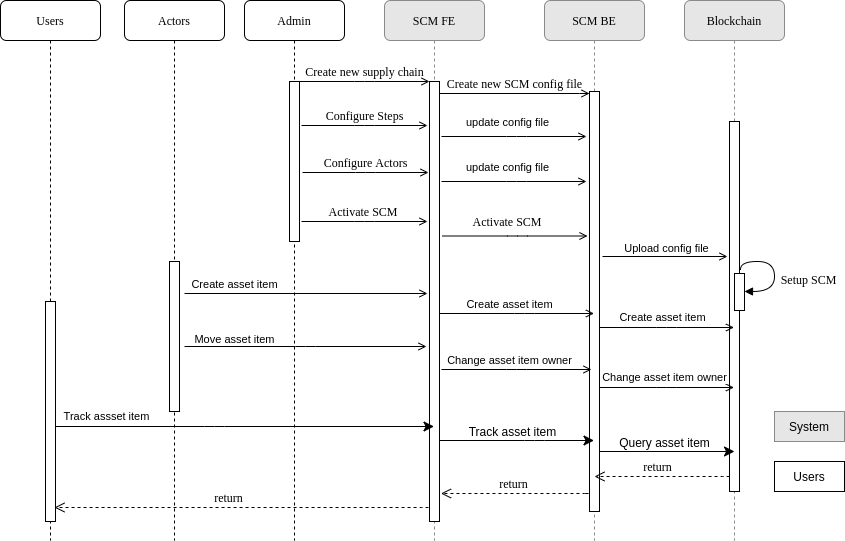
\includegraphics[scale=0.5]{images/SequenceDiagram.png}
\caption{SCM User flow}
\label{fig:sequenceDiagram}
\end{center}
\end{figure}